\documentclass[twocolumn]{article}

\usepackage{color}
\usepackage[margin=1in,bottom=1.5in]{geometry}

\usepackage{graphicx}
\usepackage{amsmath}
\usepackage{subcaption}

% Comment out second line to disable.
% Thanks: https://gist.github.com/orbekk/1298622
\newcommand{\todo}[1]{}
\renewcommand{\todo}[1]{{\color{red} TODO: {#1}}}

\newcommand{\secref}[1]{Section~\ref{sec:#1}}
\newcommand{\seclab}[1]{\label{sec:#1}}
\newcommand{\figref}[1]{Figure~\ref{fig:#1}}
\newcommand{\figlab}[1]{\label{fig:#1}}
\newcommand{\tblref}[1]{Table~\ref{tbl:#1}}
\newcommand{\tbllab}[1]{\label{tbl:#1}}

\title{Modeling Image Segmentation as Epidemic Spread in an Interdependent Network}
\author{
  Connor Greenwell, Emory Hufbauer\\
  Computer Science Dept. \\
  University of Kentucky
}
\date{}

\begin{document}

\maketitle

\begin{abstract}
We propose formulating the problem of image segmentation as a form of phenomena spread on an interdependent network of superpixels. We define two independent metrics for superpixel similarity and use them to generate two unique, but connected topologies describing the image. We then model image segmentation as the spread of the phenomenon of similarity, using two different propagation models. We then extensively optimize these models against the PASCAL VOC training dataset. Finally we compare our method against a clustering-based baseline algorithm operating on the same superpixelizations.
\end{abstract}

\section{Introduction}

Image segmentation is an important and popular topic in computer vision \cite{newell2017associative, li2017fully, ren2017end}. It is important to note that image segmentation is a distinct but related task to object detection. Notably, image segmentation is not concerned with \emph{what} the objects in an image might be, only \emph{where} they are. Typically this is formulated as assigning a unique label to each pixel in an image, where the label indicates belonging to a particular object. For example, an image containing two cats would be expected to have three labels: one for each cat, and a background label. The current state of the art uses convolutional neural networks.

Interdependent network theory is the branch of network theory devoted to studying the behavior and properties of networks composed of two or more sub-networks, each with different topology or complex interactions. Interdependent network theory is commonly used for analyzing the propagation of phenomena like power failure or social influence through complex networks such as cyber-physical systems and social networks. We propose an interdependent network model of image topology, and explore the use of propagation models to segment the image. 

\subsection{Related Work}\seclab{related}

\cite{son2012percolation} establishes theory for talking about epidemic spread
in interdependent graphs. \cite{pastor2015epidemic, pellis2015eight} deals more
specifically with epidemic spread in complex networks.
\cite{boccaletti2014structure, kivela2014multilayer} deals more broadly with the
dynamics of interdependent graphs.

\cite{pei2014saliency} use a Markov-Random-Field on precomputed super pixels to
perform image segmentation.  \cite{newell2017associative, li2017fully,
ren2017end} present a variety of neural network based approached to instance
segmentation on natural images.

\section{Approach}\seclab{approach}

\subsection{Image Network Extraction}

To construct our interdependent network model of image topology, first we apply an established superpixelization algorithm (specifically SLIC0) to the image, clustering nearby pixels together into contiguous regions.

Because superpixelization groups similar pixels together, we can approximate the topology of the underlying image using the superpixel network, greatly simplifying future operations.

\subsubsection{Alpha superpixel similarity metric}

We then define two independent metrics for the similarity of a pair of superpixels. They are ultimately used to generate the topologies of the respective layers of the interdependent network model, so their mutual independence ensures the dissimilar topology of the network layers.

The first metric (the alpha metric) measures the difference in average value (or "brightness") between a pair of superpixels. Initially, each pixel in the image is represented as an RGB color vector $x$. The alpha metric first computes the euclidean norm of each pixel's vector, and normalizes the result to the range $[0, 1]$. The result is a measure of the pixel's brightness which is independent of its hue or saturation:
\[
    \alpha_p(\underbar{x}) = \frac{\underbar{x} \cdot \underbar{x}}{\sqrt{3}} = \frac{1}{\sqrt{3}}(\underbar{x}_r^2+\underbar{x}_g^2+\underbar{x}_b^2)
\]

For a pair of superpixels $X$ and $Y$, we then define the alpha metric to be the normalized reciprocal of the absolute value of the difference between the average values of the pixels in each:
\[
    \alpha(X,\: Y) = \frac{2}{1 + \lvert \bar{X}_\alpha - \bar{Y}_\alpha \rvert} - 1
\]
\[
    \bar{X}_\alpha = \sum\limits_{\underbar{x}\: \in\: X} \alpha_p(\underbar{x}),\ \bar{Y}_\alpha = \sum\limits_{\underbar{y}\: \in\: Y} \alpha_p(\underbar{y})
\]

The result is a real value in the range $[0, 1]$, with lower values representing less similar superpixels.

\subsubsection{Beta superpixel similarity metric}

The second (or "beta") superpixel similarity metric instead rejects value information entirely, and measures the similarity in saturation and hue between two superpixels. First, it subtracts the vector $[0.5, 0.5, 0.5]$ from the each pixel's color vector, and then divides it by it's own magnitude:
\[
    \beta_p(\underbar{x}) = \frac{\underbar{x} - [0.5, 0.5, 0.5]}{\lvert \underbar{x} - [0.5, 0.5, 0.5] \rvert}
\]

This effectively transforms the color space from the cube between $[0, 0, 0] -> [1, 1, 1]$, to the hollow sphere with radius $1$ and centered at the origin. Points on the surface of the sphere represent unique saturation/value combinations. We then average and renormalize these vectors for each superpixel, and take the dot product between them. Because their magnitudes are unit, the dot product effectively measures the cosine of the average angle between the two superpixels in saturation/value space. We finally normalize to the range $[0, 1]$:
\[
    \beta(X,\: Y) = \frac{1}{2}[1 + \bar{X}_\beta \cdot \bar{Y}_\beta]
\]
\[
    \bar{X}_\beta = \sum\limits_{\underbar{x}\: \in\: X} \beta_p(\underbar{x}),\ \bar{Y}_\beta = \sum\limits_{\underbar{y}\: \in\: Y} \beta_p(\underbar{y})
\]

\begin{figure}[h]
  \centering
  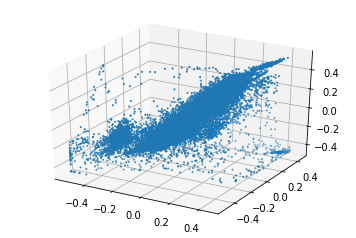
\includegraphics[width=0.45\linewidth]{figs/cloud.png}
  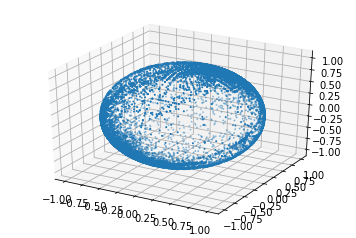
\includegraphics[width=0.45\linewidth]{figs/sphere.png}
  \caption{
    The color space before (left) and after (right) transformation to the sphere
  }
\end{figure}

\subsubsection{Constructing the network}

Next, for each layer we construct the adjacency network over the set of superpixels, and assign weights to its edges based on the above metrics. The result is an $\alpha$ layer and a $\beta$ layer, which share the same structure, but have independent weightings.

\begin{figure}[h]
  \centering
  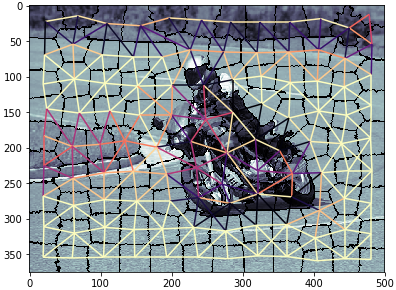
\includegraphics[width=0.49\linewidth]{figs/alpha_graph.png}
  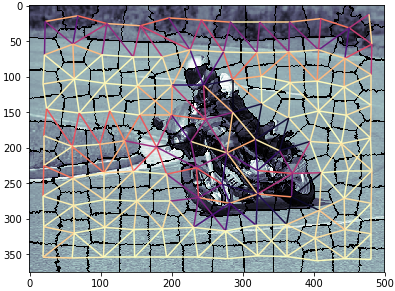
\includegraphics[width=0.49\linewidth]{figs/beta_graph.png}
  \caption{
    The two layers ($\alpha$ left, $\beta$ right) of our network model for a sample image
  }
  \figlab{ab_graph}
\end{figure}

The two layers are then connected one-to-one to form a single network model.

\subsection{Propagation}

Finally, we are able to perform propagation. We used two models: a markov random-walk model, and a weighted SI-model.


\begin{figure*}[t]
  \centering

  \begin{subfigure}{0.49\linewidth}
    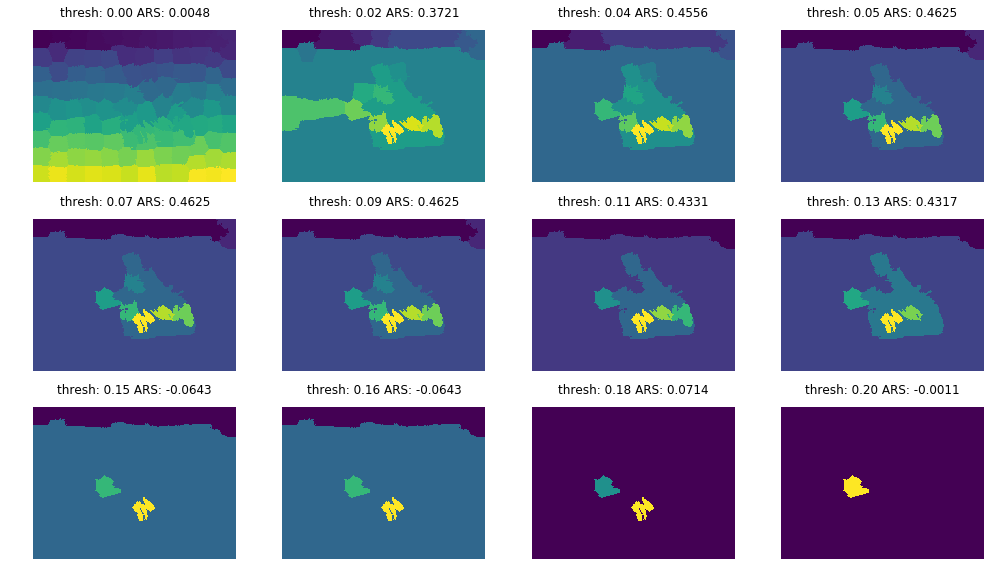
\includegraphics[width=\linewidth]{figs/only_alpha.png}
    \caption{Sample segmentation using only the alpha scores.}
  \end{subfigure}
  \begin{subfigure}{0.49\linewidth}
    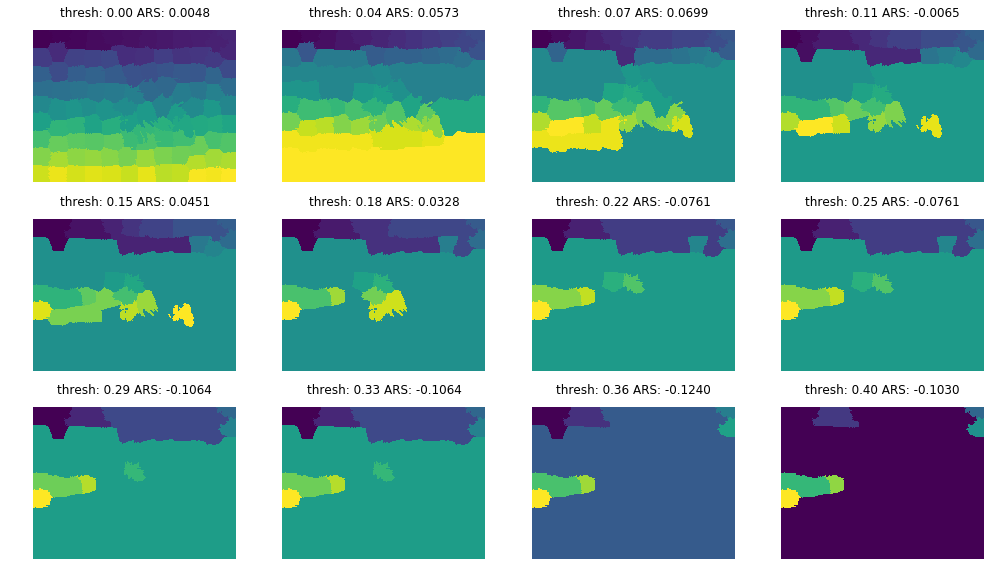
\includegraphics[width=\linewidth]{figs/only_beta.png}
    \caption{Sample segmentation using only the beta scores.}
  \end{subfigure}

  \caption{
    Each of our proposed similarity metrics provides enough information to
    perform rudamentary segmentation. To demonstrate this we take a simple
    thresholding approach, cutting edges below a given threshold, shown above
    each image. 
    We observe that in this setting, alpha scores seem useful for
    differentiating between regions in the foreground, and beta scores seem
    useful for regions in the background. Our intuition is that combining these
    two metrics will yield superior segmentations.
  }
  \figlab{ab_only}
\end{figure*}

\subsection{Baseline}

A naive baseline method has been developed for us to compare our actual method
against. It is based on using DBSCAN \cite{ester1996density} to cluster and
merge superpixels produced by SLIC \cite{achanta2010slic}.

\subsection{Dataset}\seclab{data}

The dataset upon which we evaluate our method is the PASCAL Visual Object
Classification (VOC) dataset \cite{Everingham10}. Over the years in which the
VOC challenge was run, a couple different variations of the problem we
presented, ranging from whole-image object classification to human pose
estimation. In 2012 they introduced a subset of per-pixel image segmentations
for $2,913$ of the images in the dataset. In each segmentation, there is a
background class, some number of instance classes, and a "don't care" region
around each object instance. The image segmentation task is distinct from
object classification in that the goal is not to actually classify to which
object category each pixel belongs to, but to separate the image into its
constituent parts, similar to foreground/background segmentation. We believe
that this task presents a unique challenge that can be addressed by our proposed
method of propagating information through a interdependent graph defined by
pixel/region similarities.

\section{Results and Discussion}\seclab{results}

\begin{figure}[t]
  \centering
  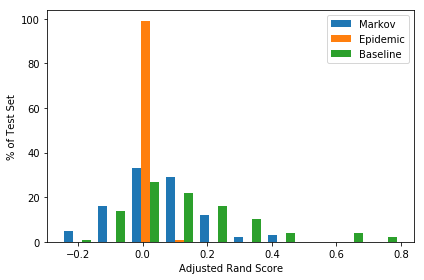
\includegraphics[width=\linewidth]{figs/bars.png}
  \caption{Comparison of Adjusted Rand Score on 100 images from the training
  set. Having more area to the right of the graph indicates a higher proportion
  of high quality seqmentations. In this case, this indicates that our method is
  worse than our defined baseline.
  }
  \figlab{bars}
\end{figure}

We evaluate our methods on the Adjusted Rand Score (ARS) from
\cite{unnikrishnan2005measure}. In \figref{bars} we visualize the distribution
of ARS for each of our described methods (baseline, Markov-based, and
Epidemic-based). In \tblref{ars} we show the average ARS of each method on the
PASCAL VOC dataset. Both of the methods proposed in this paper perform worse
than the baseline; quantitatively, qualitatively, and in terms of computation
time.

\begin{table}
    \centering
    \caption{Mean Adjusted Rand Score for each method covered in this paper.
    Higher values indicicate higher quality segmentations.}
    \tbllab{ars}

    \begin{tabular}{c|l}
        Method & Mean ARS \\ \hline
        Baseline & 0.1385439 \\
        Markov-based & 0.0536634 \\
        Epidemic-based & 0.0124122
    \end{tabular}
\end{table}

\begin{figure}[t!]
\centering

  \begin{subfigure}{\linewidth}
    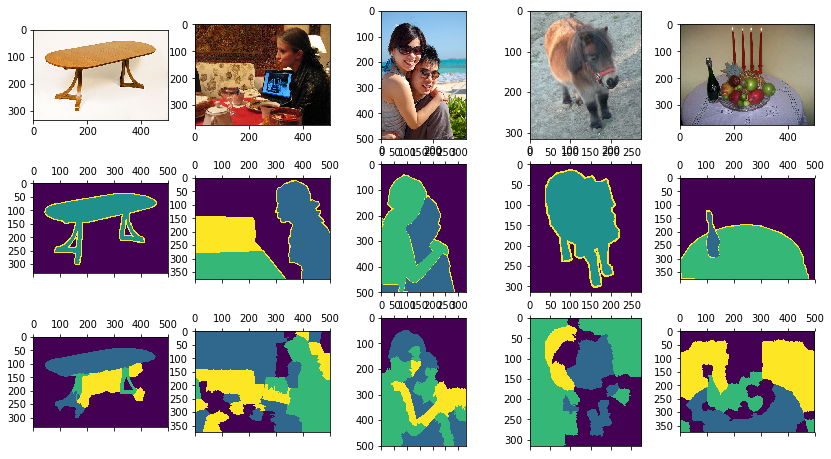
\includegraphics[width=\linewidth]{figs/baseline_best.png}
    \caption{Baseline}
  \end{subfigure}

  \begin{subfigure}{\linewidth}
    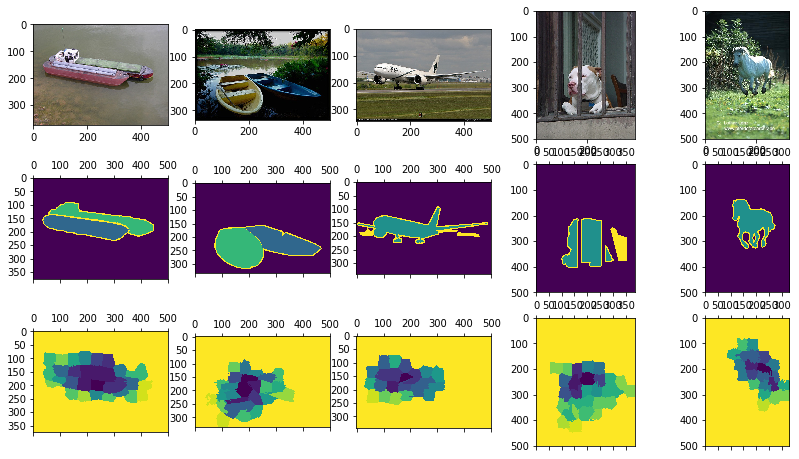
\includegraphics[width=\linewidth]{figs/markov_best.png}
    \caption{Markov random walk based}
  \end{subfigure}

  \begin{subfigure}{\linewidth}
    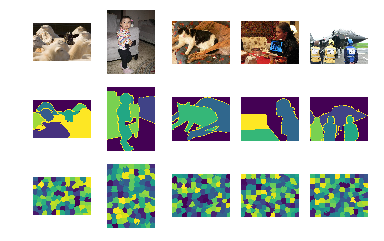
\includegraphics[width=\linewidth]{figs/epidemic_best.png}
    \caption{Epidemic based}
  \end{subfigure}

\caption{Sample results from each of our proposed methods.}
\figlab{sample_results}
\end{figure}

Qualitatively, segmentations produced by the Markov-based and Epidemic-based
methods leave much to be desired. \figref{sample_results} shows the images and
resulting segmentations for the five highest scoring images under each method.
The Markov-based segmentations are noisy and typically centered over points of
interest in an image. This noise can be attributed to the fact that the
likelyhood of arriving in a particular node during a random walk is not uniform
when starting in other nodes in a single object. 

\begin{figure*}[t!]
  \centering

  \begin{subfigure}{0.49\linewidth}
    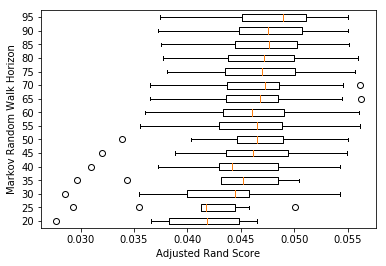
\includegraphics[width=\linewidth]{figs/markov_horizon.png}
    \caption{Markov random walk, walk horizon}
  \end{subfigure}
  \begin{subfigure}{0.49\linewidth}
    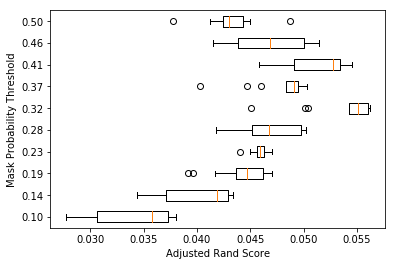
\includegraphics[width=\linewidth]{figs/markov_thresh.png}
    \caption{Markov random walk, merge threshold}
  \end{subfigure}

  \begin{subfigure}{0.49\linewidth}
    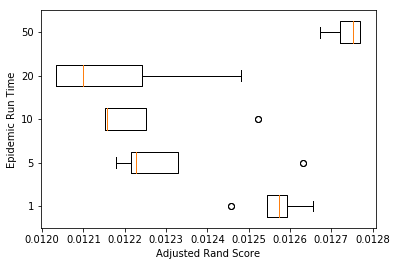
\includegraphics[width=\linewidth]{figs/epidemic_run.png}
    \caption{Epidemic, simulation runtime}
  \end{subfigure}
  \begin{subfigure}{0.49\linewidth}
    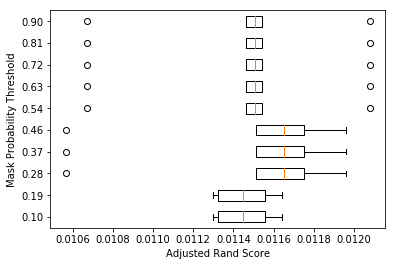
\includegraphics[width=\linewidth]{figs/epidemic_thresh.png}
    \caption{Epidemic, merge threshold}
  \end{subfigure}

  \caption{
    Analysis of performance under different hyperparameters for each of our
    proposed methods. (a) and (b) show that threshold is the most important
    parameter for the Markov-based method. (c) and (d) show that simulation run
    time is the most important parameter for the Epidemic-based method.
  }
  \figlab{param_sweep}

\end{figure*}

Each method described is subject to a number of hyperparameters which ultimately 
dictate the methods performance with regards to ARS. In \figref{param_sweep} we
show the results of a hyperparameter sweep over both the Markov-based and
Epidemic-based methods. They share the a parameter controling the threshold at
which each proposed segmentation is binarized at. Interestingly, each method
demonstrates its own sensitiveity to the parameter. Specificly, the Epidemic
model is relatively insensitive to it. We attribute this to a quirk of the
Epidemic-based method, proposal segmentations that begin in areas with low
neighboring similarity will not spread far. Due to the way that we combine
proposed segmentations, this produces many smaller, less informative segments.
Effectively we are amplifying noise in the signal. In \figref{epidemic_only} we
demonstrate what happens when we use a simple heuristic to select the best
proposals.

\begin{figure}[t]
    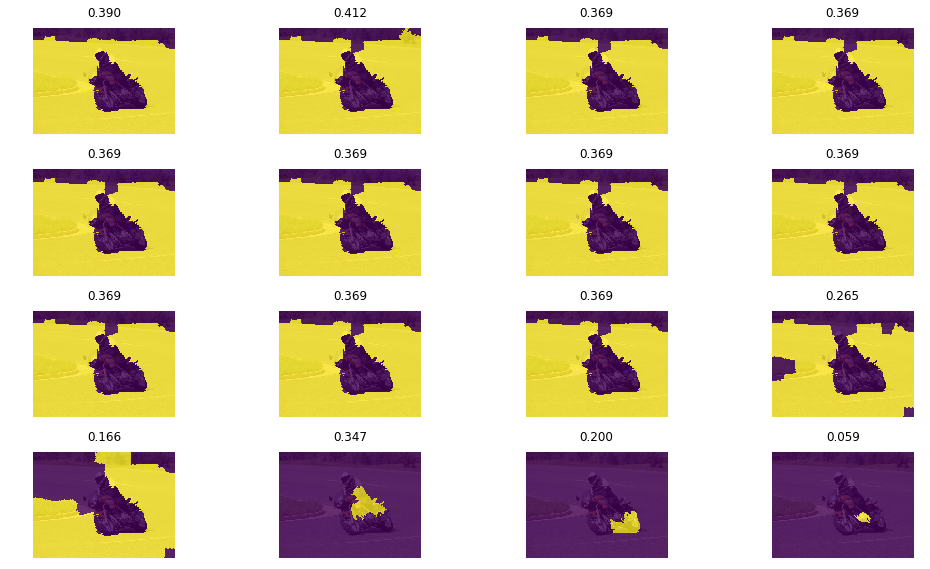
\includegraphics[width=\linewidth]{figs/epidemic_heuristic.png}
    \caption{Binaried segmentations proposed by the epidemic-based method,
    sorted by our simple heuristic.}
    \figlab{epidemic_only}
\end{figure}

\section{Conclusion}

In this document we presented a method for performing instance segmentation on
photographs by modeling instance membership as an information spread or epidemic
model in an interdependent graph. We introduced two simple similarity metrics
which are used as the basis for tranmitting instance membership between
neighboring pixels. Finally we compare our method to a rudamentary baseline.

\subsection{Future Work}

These methods did not perform better than the proposed baseline. Some possible
directions for future work include the following:

\begin{itemize}
  \item Improving the method by which we combine candidate segmentations.
  \item Incorporating additional similarity metrics, and additional layers to the interdependent graph.
  \item Explore the effect of using other superpixel segmentation strategies.
\end{itemize}

\bibliographystyle{plain}
\bibliography{refs} 

\end{document}
